\documentclass[11pt,article]{memoir}
\usepackage{multirow}
\usepackage{agd-assignment}
\usepackage{fancybox}
\usepackage{afterpage}
\usepackage{graphicx}
\usepackage{standalone}
\usepackage[yyyymmdd,hhmmss]{datetime}


\usepackage{listings}
\lstset{
    frame=single,
    breaklines=true,
    postbreak=\raisebox{0ex}[0ex][0ex]{\ensuremath{\color{red}\hookrightarrow\space}}
}
\let\footruleskip\undefined
\usepackage{fancyhdr}
\fancyhf{}
\lhead{\textbf{FRCRCE}}
\rhead{\textbf{DEPARTMENT OF INFORMATION TECHNOLOGY}}

\rfoot{Compiled on \today\ at \currenttime \quad \textbf{\thepage}}
%\pagestyle{fancy}
\assigncourse{Course title: Big Data Analytics}
\assignterm{Course term: 2019-2020}
\assigncat{Practical}
%\assigntitle{}
%\renewcommand{\headrulewidth}{0pt}
%\renewcommand{\footrulewidth}{0pt}}
\lfoot{\textbf{Course title: Big Data Analytics}}

\fancypagestyle{plain}{}
\pagestyle{fancy}
\begin{document}
\sloppy
\fancypage{\doublebox}{}
\begin{flushleft}


    \begin{tabular}{ | p{4cm} | p{5cm} | p{3.5cm} | p{2cm} |}
    \hline

    \textbf{Name of the student:}& Tanmay Prashant Rane &\textbf{Roll No.} & 8031 \\ \hline
    \textbf{Practical Number:}& 8 & \textbf{Date of Practical:} & \\ \hline
	\textbf{Relevant CO's} & \multicolumn{3}{|p{10.5cm}|}{\begin{flushleft}
	\textbf{At the end of the course students will be able to apply appropriate algorithms for extracting knowledge from given dataset.}
	\end{flushleft}}\\
    \hline
    \multicolumn{3}{|p{12.5cm}|}{\textbf{Sign here to indicate that you have read all the relevant material provided before attempting this practical}}& \textbf{Sign:}\\ \hline
    \end{tabular}
    \vspace{1cm}
        \textbf{Practical grading using Rubrics}
           \begin{tabular}{|p{2cm}|p{2cm}|p{2cm}|p{2cm}|p{2cm}|p{2cm}|}
           \hline \textbf{Indicator} & \textbf{Very Poor} & \textbf{Poor} & \textbf{Average} & \textbf{Good} & \textbf{Excellent} \\ 
           \hline \textbf{Timeline} (2) & Practical not submitted (0) & More than two session late (0.5) & Two sessions late (1) & One session late (1.5) & Early or on time (2) \\ 
           \hline \textbf{Code design} (3) & N/A & Very poor code design(0) & poor design (1) & design with good coding standards (2) & Accurate Design with better coding standards(3) \\ 
           \hline \textbf{Execution} (3) & N/A & Very less execution (0)
            & little execution.(1) & Major execution(2)
            & Entire code execution (3) \\ 
           \hline \textbf{Postlab} (2) & Both answers wrong(0) & N/A& One answer correct (1) & N/A & Both answers correct (2) \\ 
           \hline 
           \end{tabular}
        \vspace{-8cm}
        \begin{table}[h!]
        \centering
        \begin{tabular}{|c|c|}
                \hline \textbf{Total Marks (10)} & \textbf{Sign of instructor with date} \\ 
                \hline  &  \\ & \\
                \hline 
                \end{tabular} 
        \end{table}
        
    \pagebreak

	%\input{assignment}

\maketitle

%\thispagestyle{empty}
\hrule \vspace{0.2cm}
\textbf{Problem Statement: To implement kNN algorithm using map-reduce. }\hrule\vspace{0.2cm}
\textbf{Theory:}\hrule\vspace{0.2cm}
%
The k – Nearest Neighbor Algorithm
The k-Nearest Neighbor Algorithm involves two phases.
• The Training Phase
• The Testing Phase
These Phases are discussed in detail in the following subsections.
1) The Training Phase
kNN Algorithm does not explicitly require any training phase for the data to be classified. The training phase usually
involves storing the data vector co-ordinates along with the class label. The class label in general is used as an identifier
for the data vector. This is used to classify data vectors during the testing phase
2) The Testing Phase Given data points for testing, our aim is to find the class label for the new point. The algorithm is discussed for k=1 or 1 Nearest Neighbor rule and then extended for k=k or kNearest Neighbor rule.
a) k=1 or 1 Nearest Neighbor
This is the simplest scenario for classification. Let ‘x’ be the point to be labeled.
• Find the point closest to ‘x’ in the training data set.
Let this closest point be ‘y’.
• Now nearest neighbor rule asks to assign the label of
‘y’ to ‘x’.
This seems too simplistic and some times even counter intuitive. This reasoning holds only when the number of data points is not very large. If the number of data points is very large, then there is a very high chance that label of x and y are same. \\
\parskip 5mm
b) k=K or k-Nearest Neighbor
This is a direct extension of 1NN. ’k’ nearest neighbors are found for a given data point from the testing data set and a it is classified by a majority vote conducted in the training data set. Typically ‘k’ is odd when the number of classes is 2.
Here is an example to illustrate the majority voting. Consider a data point belonging to the testing data set. Let k =
5 and the training data set in the vicinity of the data point to be classified are 3 data points with class label C1 and 2 data points with class label C2. In this case, according to kNN the new data point will have the label as C1 as it forms the
majority. Similar argument when there are multiple classes.\linebreak
\\
3) Generalising the k-Nearest Neighbor Testing Phase \\
1. Determine the value of ‘k’ (input) \linebreak
2. Prepare the training data set by storing the coordinates and class labels of the data points. \linebreak
3. Load the data point from the testing data set.\linebreak
4. Conduct a majority vote amongst the ‘k’ closest
neighbors of the testing data point from the training
data set based on a distance metric.\linebreak
5. Assign the class label of the majority vote winner to
the new data point from the testing data set.\linebreak
6. Repeat this until all the Data points in the testing
phase are classified.\linebreak

	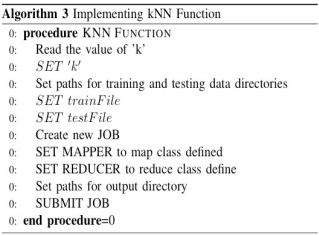
\includegraphics{driver.png}
	
	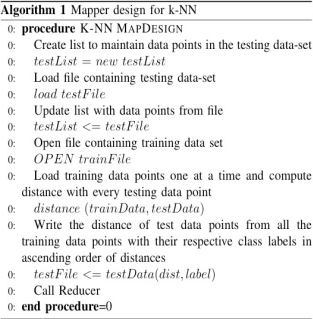
\includegraphics{map.png}

	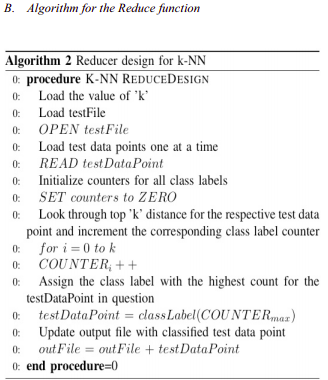
\includegraphics{reduce.png}
\afterpage{\newpage}\newpage
\textbf{Code:}\hrule
\vspace{0.5cm}
Write map-reduce code to implement kNN algorithm. Use CarOwners.csv as input file to train the model. Take the following tuple as input from the user and try classifying it using kNN.\\
Test tuple to be taken as input from the user: k=5, Age=67, income=16668, Status=Single, Gender=Male, Children=3.\\
\textbf{\underline{code for mapper:}}

% Write code of mapper here
\begin{lstlisting}[language=java]

import java.io.DataInput;
import java.io.DataOutput;
import java.io.IOException;
import java.io.File;
import java.net.URI;
import java.util.ArrayList;
import java.util.HashMap;
import java.util.List;
import java.util.Map;
import java.util.StringTokenizer;
import java.util.TreeMap;

import org.apache.commons.io.FileUtils;
import org.apache.hadoop.conf.Configuration;
import org.apache.hadoop.fs.Path;
import org.apache.hadoop.io.NullWritable;
import org.apache.hadoop.io.Text;
import org.apache.hadoop.io.WritableComparable;
import org.apache.hadoop.mapreduce.Job;
import org.apache.hadoop.mapreduce.Mapper;
import org.apache.hadoop.mapreduce.Reducer;
import org.apache.hadoop.mapreduce.lib.input.FileInputFormat;
import org.apache.hadoop.mapreduce.lib.output.FileOutputFormat;
public class KnnMapper extends Mapper<Object, Text, NullWritable, DoubleString>
{
DoubleString distanceAndModel = new DoubleString();
TreeMap<Double, String> KnnMap = new TreeMap<Double, String>();

// Declaring some variables which will be used throughout the mapper
int K;
double normalisedSAge;
double normalisedSIncome;
String sStatus;
String sGender;
double normalisedSChildren;

// The known ranges of the dataset, which can be hardcoded in for the purposes of this example
double minAge = 18;
double maxAge = 77;
double minIncome = 5000;
double maxIncome = 67789;
double minChildren = 0;
double maxChildren = 5;

// Takes a string and two double values. Converts string to a double and normalises it to
// a value in the range supplied to reurn a double between 0.0 and 1.0 
private double normalisedDouble(String n1, double minValue, double maxValue)
{
return (Double.parseDouble(n1) - minValue) / (maxValue - minValue);
}

// Takes two strings and simply compares then to return a double of 0.0 (non-identical) or 1.0 (identical).
// This provides a way of evaluating a numerical distance between two nominal values.
private double nominalDistance(String t1, String t2)
{
if (t1.equals(t2))
{
return 0;
}
else
{
return 1;
}
}

// Takes a double and returns its squared value.
private double squaredDistance(double n1)
{
return Math.pow(n1,2);
}


// Takes ten pairs of values (three pairs of doubles and two of strings), finds the difference between the members
// of each pair (using nominalDistance() for strings) and returns the sum of the squared differences as a double.
private double totalSquaredDistance(double R1, double R2, String R3, String R4, double R5, double S1,
double S2, String S3, String S4, double S5)
{	
double ageDifference = S1 - R1;
double incomeDifference = S2 - R2;
double statusDifference = nominalDistance(S3, R3);
double genderDifference = nominalDistance(S4, R4);
double childrenDifference = S5 - R5;

// The sum of squared distances is used rather than the euclidean distance
// because taking the square root would not change the order.
// Status and gender are not squared because they are always 0 or 1.
return squaredDistance(ageDifference) + squaredDistance(incomeDifference) + statusDifference + genderDifference + squaredDistance(childrenDifference);
}

// The @Override annotation causes the compiler to check if a method is actually being overridden
// (a warning would be produced in case of a typo or incorrectly matched parameters)
@Override
// The setup() method is run once at the start of the mapper and is supplied with MapReduce's
// context object
protected void setup(Context context) throws IOException, InterruptedException
{
if (context.getCacheFiles() != null && context.getCacheFiles().length > 0)
{
// Read parameter file using alias established in main()
String knnParams = FileUtils.readFileToString(new File("./knnParamFile"));
StringTokenizer st = new StringTokenizer(knnParams, ",");

// Using the variables declared earlier, values are assigned to K and to the test dataset, S.
// These values will remain unchanged throughout the mapper
K = Integer.parseInt(st.nextToken());
//				System.out.println(K);
normalisedSAge = normalisedDouble(st.nextToken(), minAge, maxAge);
normalisedSIncome = normalisedDouble(st.nextToken(), minIncome, maxIncome);
sStatus = st.nextToken();
sGender = st.nextToken();
normalisedSChildren = normalisedDouble(st.nextToken(), minChildren, maxChildren);
}
}

@Override
// The map() method is run by MapReduce once for each row supplied as the input data
public void map(Object key, Text value, Context context) throws IOException, InterruptedException
{
// Tokenize the input line (presented as 'value' by MapReduce) from the csv file
// This is the training dataset, R
String rLine = value.toString();
//			System.out.println("Hello Mapper");
StringTokenizer st = new StringTokenizer(rLine, ",");

double normalisedRAge = normalisedDouble(st.nextToken(), minAge, maxAge);
double normalisedRIncome = normalisedDouble(st.nextToken(), minIncome, maxIncome);
String rStatus = st.nextToken();
String rGender = st.nextToken();
double normalisedRChildren = normalisedDouble(st.nextToken(), minChildren, maxChildren);
String rModel = st.nextToken();

// Using these row specific values and the unchanging S dataset values, calculate a total squared
// distance between each pair of corresponding values.
double tDist = totalSquaredDistance(normalisedRAge, normalisedRIncome, rStatus, rGender,
normalisedRChildren, normalisedSAge, normalisedSIncome, sStatus, sGender, normalisedSChildren);		

// Add the total distance and corresponding car model for this row into the TreeMap with distance
// as key and model as value.
KnnMap.put(tDist, rModel);
// Only K distances are required, so if the TreeMap contains over K entries, remove the last one
// which will be the highest distance number.
if (KnnMap.size() > K)
{
KnnMap.remove(KnnMap.lastKey());
}
}

@Override
// The cleanup() method is run once after map() has run for every row
protected void cleanup(Context context) throws IOException, InterruptedException
{
// Loop through the K key:values in the TreeMap
for(Map.Entry<Double, String> entry : KnnMap.entrySet())
{
Double knnDist = entry.getKey();
String knnModel = entry.getValue();
// distanceAndModel is the instance of DoubleString declared aerlier
distanceAndModel.set(knnDist, knnModel);
// Write to context a NullWritable as key and distanceAndModel as value
context.write(NullWritable.get(), distanceAndModel);
}
}
}
	
\end{lstlisting}

\textbf{\underline{Code for Reducer:}}
\begin{lstlisting}[language=java]
public class KnnReducer extends Reducer<NullWritable, DoubleString, NullWritable, Text>
{
TreeMap<Double, String> KnnMap = new TreeMap<Double, String>();
int K;

@Override
// setup() again is run before the main reduce() method
protected void setup(Context context) throws IOException, InterruptedException
{
if (context.getCacheFiles() != null && context.getCacheFiles().length > 0)
{
// Read parameter file using alias established in main()
String knnParams = FileUtils.readFileToString(new File("./knnParamFile"));
StringTokenizer st = new StringTokenizer(knnParams, ",");
// Only K is needed from the parameter file by the reducer
K = Integer.parseInt(st.nextToken());
}
}

@Override
// The reduce() method accepts the objects the mapper wrote to context: a NullWritable and a DoubleString
public void reduce(NullWritable key, Iterable<DoubleString> values, Context context) throws IOException, InterruptedException
{
// values are the K DoubleString objects which the mapper wrote to context
// Loop through these
for (DoubleString val : values)
{
String rModel = val.getModel();
double tDist = val.getDistance();

// Populate another TreeMap with the distance and model information extracted from the
// DoubleString objects and trim it to size K as before.
KnnMap.put(tDist, rModel);
if (KnnMap.size() > K)
{
KnnMap.remove(KnnMap.lastKey());
}
}	

// This section determines which of the K values (models) in the TreeMap occurs most frequently
// by means of constructing an intermediate ArrayList and HashMap.

// A List of all the values in the TreeMap.
List<String> knnList = new ArrayList<String>(KnnMap.values());

Map<String, Integer> freqMap = new HashMap<String, Integer>();

// Add the members of the list to the HashMap as keys and the number of times each occurs
// (frequency) as values
for(int i=0; i< knnList.size(); i++)
{  
Integer frequency = freqMap.get(knnList.get(i));
if(frequency == null)
{
freqMap.put(knnList.get(i), 1);
} else
{
freqMap.put(knnList.get(i), frequency+1);
}
}

// Examine the HashMap to determine which key (model) has the highest value (frequency)
String mostCommonModel = null;
int maxFrequency = -1;
for(Map.Entry<String, Integer> entry: freqMap.entrySet())
{
if(entry.getValue() > maxFrequency)
{
mostCommonModel = entry.getKey();
maxFrequency = entry.getValue();
}
}

// Finally write to context another NullWritable as key and the most common model just counted as value.
System.out.println("Hello Reducer");
//			context.write(NullWritable.get(), new Text(mostCommonModel)); // Use this line to produce a single classification
context.write(NullWritable.get(), new Text(KnnMap.toString()));	// Use this line to see all K nearest neighbours and distances
}
}

\end{lstlisting}

\textbf{\underline{Code for Driver Class:}}
\begin{lstlisting}[language=java]
public class knndriver {

public static void main(String[] args) throws Exception
{
// Create configuration
Configuration conf = new Configuration();

//		if (args.length != 3)
//		{
//			System.err.println("Usage: KnnPattern <in> <out> <parameter file>");
//			System.exit(2);
//		}

// Create job
Job job = Job.getInstance(conf, "Find K-Nearest Neighbour");
job.setJarByClass(knndriver.class);
// Set the third parameter when running the job to be the parameter file and give it an alias
job.addCacheFile(new URI(args[0]+"#knnParamFile")); // Parameter file containing test data
//		GenericOptionsParser parser = new GenericOptionsParser(conf, args);
//		args = parser.getRemainingArgs();
// Setup MapReduce job
job.setMapperClass(KnnMapper.class);
job.setReducerClass(KnnReducer.class);
job.setNumReduceTasks(1); // Only one reducer in this design

// Specify key / value
job.setMapOutputKeyClass(NullWritable.class);
job.setMapOutputValueClass(DoubleString.class);
job.setOutputKeyClass(NullWritable.class);
job.setOutputValueClass(Text.class);

// Input (the data file) and Output (the resulting classification)
FileInputFormat.setInputPaths(job, new Path("/media/tanmay/Data/SEM-8/BDA/EXP8/Exp8bda1920/CarOwners.csv"));
FileOutputFormat.setOutputPath(job, new Path("/media/tanmay/Data/SEM-8/BDA/EXP8/Exp8bda1920/out"));

// Execute job and return status
System.exit(job.waitForCompletion(true) ? 0 : 1);
}

}

public class DoubleString implements WritableComparable<DoubleString>
{
private Double distance = 0.0;
private String model = null;

public void set(Double lhs, String rhs)
{
distance = lhs;
model = rhs;
}

public Double getDistance()
{
return distance;
}

public String getModel()
{
return model;
}

@Override
public void readFields(DataInput in) throws IOException
{
distance = in.readDouble();
model = in.readUTF();
}

@Override
public void write(DataOutput out) throws IOException
{
out.writeDouble(distance);
out.writeUTF(model);
}

@Override
public int compareTo(DoubleString o)
{
return (this.model).compareTo(o.model);
}
}
\end{lstlisting}

\noindent \textbf{Output: }\\
\parskip 10mm
\noindent \textbf{\{2.0=Zafira, 2.001118252711201=Corsa, 2.001208759634182=Corsa, 2.0012388931154517=Corsa, 2.0013956914677253=Zafira\}}



\newpage
\textbf{PostLab:}\hrule
Try using k=3 in above code. Comment on the observation made.\\
\hrule
\textbf{\underline{Answer for postlab question}} \\                       
\noindent \textbf{Output: }
\parskip 10mm

\noindent \textbf{\{2.0=Zafira, 2.001118252711201=Corsa, 2.001208759634182=Corsa\}}


\noindent When k is 3 the top 3 neighbours of the given input wiz(3, 67, 16668, Single, Male, 3) are shown, the observation is the the distance between neighbours is in  ascending order so the closest one is first in the output. So given the characteristics of person in input the cars suggested are Zafira and Corsa           
\newpage
Try using k=7 in above code. Comment on the observation made.\\
\hrule
\textbf{\underline{Answer for postlab question}}\\
\noindent \textbf{Output: }
\parskip 10mm

\noindent \textbf{\{2.0=Zafira, 2.001118252711201=Corsa, 2.001208759634182=Corsa, 2.0012388931154517=Corsa, 2.0013956914677253=Zafira, 2.002715498542882=Zafira, 2.0033228274436796=Corsa\}}

\noindent When k is 7 the top 7 neighbours of the given input wiz(7, 67, 16668, Single, Male, 3) are shown, the observation is the the distance between neighbours is in  ascending order so the closest one is first in the output. So given the characteristics of person in input the cars suggested are Zafira and Corsa and they can be seen repetitively because all nearest neighbours fetched are owners of Zafira and Corsa.     
\end{flushleft}
\end{document}

